\chapter{Ligandveldtheorie en kleur}\label{ch:b2:ligand-field}

Robijn is rood en smaragd groen, en toch danken beide hun kleur aan hetzelfde ion,
\ce{Cr^3+}, waarvan enkele aluminium vervangen in korund, \ce{Al2O3}, of in
beril. Kristallen van kopersulfaat zijn diepblauw, maar het poeder dat na
verhitten overblijft, is wit. Telkens komt de kleur van elektronen die springen
tussen d-orbitalen waarvan de omringende atomen de energieën uit elkaar getrokken hebben ---
met een bedrag dat afhangt van welke atomen het ion omringen en hoe. Dit
hoofdstuk berekent die splitsing, eerst met puntladingen, daarna met \omterm{def:b2:diatomic-mos:lcao}{molecuulorbitalen};
het verklaart kleuren, magnetisme, en de \omterm{def:b2:coordination-complexes:electron-count}{18-elektronenregel} van het
vorige hoofdstuk.

\begin{recall}
\Cref{ch:b2:coordination-complexes}: $d^n$-configuraties, geometrieën, elektronentellingen.
\Cref{ch:b2:atomic-orbitals}: de vormen van de vijf d-orbitalen.
\Cref{ch:b2:fragment-orbitals}: \omterm{def:b2:fragment-orbitals:fragment}{fragmentorbitalen}. Het deel van jaar~1: absorbantie,
complementaire kleuren, ongepaarde elektronen, de regel van Hund.
\end{recall}

\begin{omfigure}
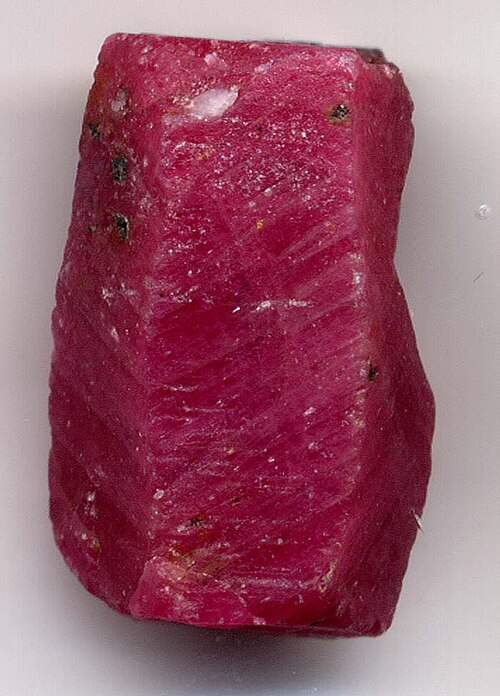
\includegraphics[height=3.6cm]{images/book3/ruby.jpg}\hspace{0.6cm}%
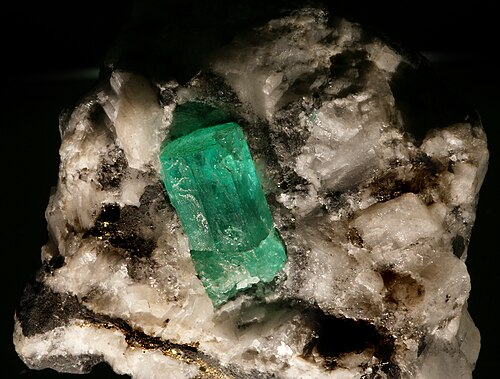
\includegraphics[height=3.6cm]{images/book3/emerald.jpg}\hspace{0.6cm}%
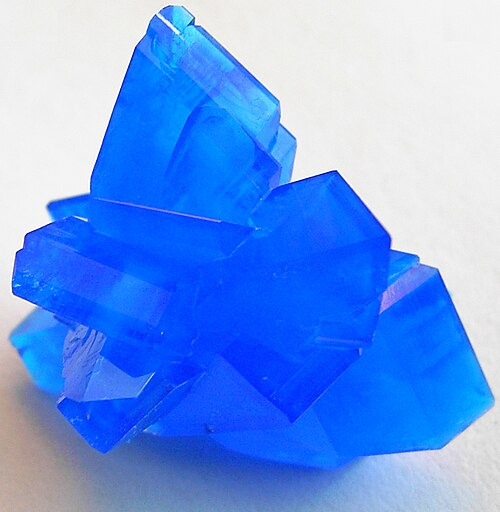
\includegraphics[height=3.6cm]{images/book3/copper-sulfate.jpg}

{\small Een robijnkristal (publiek domein); een smaragd in zijn gesteente (Didier Descouens,
CC BY-SA 3.0); kristallen van koper(II)sulfaatpentahydraat (Stephanb, CC BY-SA
3.0). Wikimedia Commons. Chroom(III) kleurt de eerste twee, het aquacomplex van
koper(II) het derde.}
\end{omfigure}

\section{Het kristalveldmodel}

\begin{definition}[Kristalveld]\label{def:b2:ligand-field:crystal-field}
Het \emph{kristalveldmodel}\index{kristalveldmodel} behandelt de liganden van een
complex als negatieve puntladingen (of de negatieve uiteinden van dipolen) rond het metaalion,
en berekent hoe ze de energieën van zijn d-orbitalen veranderen. In een octaëdrisch
veld splitsen de d-orbitalen in twee verzamelingen, gescheiden door de
\emph{kristalveldsplitsing}\index{kristalveldsplitsing} $\Delta_o$.
\end{definition}

Plaats de zes liganden op de assen. De orbitalen $\mathrm d_{z^2}$ en $\mathrm d_{x^2-y^2}$
richten hun lobben recht op liganden: een elektron erin wordt sterker afgestoten
en ze stijgen. De orbitalen $\mathrm d_{xy}$, $\mathrm d_{xz}$, $\mathrm d_{yz}$ wijzen tussen
de liganden door en stijgen minder. Het eerste paar heet $e_g$, de tweede verzameling van drie
$t_{2g}$ (namen uit de groepentheorie, in het deel van jaar~3).

\begin{omfigure}
\begin{tikzpicture}[font=\small]
  \begin{scope}
    \pic at (0,0) {omdx2y2};
    \foreach \p in {(1.25,0),(-1.25,0),(0,1.25),(0,-1.25)} \node[circle, fill=black!70, inner sep=2.2pt] at \p {};
    \node at (0,-1.75) {$\mathrm d_{x^2-y^2}$: lobben naar de liganden};
  \end{scope}
  \begin{scope}[xshift=5.5cm]
    \pic at (0,0) {omdxy};
    \foreach \p in {(1.25,0),(-1.25,0),(0,1.25),(0,-1.25)} \node[circle, fill=black!70, inner sep=2.2pt] at \p {};
    \node at (0,-1.75) {$\mathrm d_{xy}$: lobben ertussen};
  \end{scope}
\end{tikzpicture}

{\small Twee d-orbitalen tussen de vier liganden van het $xy$-vlak van een octaëder
(zwarte punten). De lobben van $\mathrm d_{x^2-y^2}$ wijzen naar de liganden, die van
$\mathrm d_{xy}$ ertussen.}
\end{omfigure}

\begin{theorem}[Zwaartepunt]\label{thm:b2:ligand-field:barycentre}
In een octaëdrisch veld ligt, gemeten vanaf de gemiddelde energie van de d-orbitalen, het
paar $e_g$ op $+0.6\Delta_o$ en de verzameling $t_{2g}$ op $-0.4\Delta_o$.
\end{theorem}

\begin{proof}
Het veld verhoogt het gemiddelde van de vijf d-energieën, maar de splitsing verandert het
niet (de zwaartepuntsregel, aangenomen: de som van de verschuivingen van een volledige verzameling
orbitalen ligt vast door de totale lading, niet door haar schikking). Met $e_g$ op $x$ en
$t_{2g}$ op $x - \Delta_o$ geeft de voorwaarde $2x + 3(x - \Delta_o) = 0$ dat $x = 0.6\Delta_o$.
\end{proof}

\section{Hoogspin en laagspin}

\begin{definition}[Spintoestanden]\label{def:b2:ligand-field:spin}
De \emph{paringsenergie}\index{paringsenergie} $P$ is de energie die nodig is om een tweede
elektron in een bezette orbitaal te plaatsen in plaats van in een lege met dezelfde energie. Een
complex is \emph{hoogspin}\index{hoogspin} wanneer zijn elektronen de $e_g$-orbitalen bezetten
voordat ze in $t_{2g}$ paren, \emph{laagspin}\index{laagspin} wanneer ze eerst in $t_{2g}$
paren.
\end{definition}

\begin{proposition}[Keuze van de spintoestand]\label{prop:b2:ligand-field:spin-state}
Voor octaëdrische ionen $d^4$ tot $d^7$ is het complex \omterm{def:b2:ligand-field:spin}{laagspin} als $\Delta_o > P$ en \omterm{def:b2:ligand-field:spin}{hoogspin}
als $\Delta_o < P$. Voor $d^1$--$d^3$ en $d^8$--$d^{10}$ bestaat er maar één configuratie.
\end{proposition}

\begin{proof}
Vanaf $d^3$ ($t_{2g}^3$) gaat het vierde elektron ofwel naar $e_g$ (kost $\Delta_o$ boven
$t_{2g}$) ofwel paart het in $t_{2g}$ (kost $P$). Het goedkoopste wint; dezelfde vergelijking geldt
voor elk elektron tot $d^7$. Voor $d^1$--$d^3$ is er plaats in $t_{2g}$ zonder paring;
voor $d^8$--$d^{10}$ is $t_{2g}$ vol en moet $e_g$ hoe dan ook gebruikt worden.
\end{proof}

\begin{definition}[Kristalveldstabilisatie-energie]\label{def:b2:ligand-field:cfse}
De \emph{kristalveldstabilisatie-energie}\index{kristalveldstabilisatie-energie}
(CFSE) van een configuratie $t_{2g}^ae_g^b$ is $(-0.4a + 0.6b)\Delta_o$, de energie van
de d-elektronen ten opzichte van het zwaartepunt (de paringsenergieën apart geteld).
\end{definition}

\begin{proposition}[CFSE langs de reeks]\label{prop:b2:ligand-field:cfse}
Bij \omterm{def:b2:ligand-field:spin}{hoogspin} is de CFSE $0$, $-0.4$, $-0.8$, $-1.2$, $-0.6$, $0$, $-0.4$, $-0.8$, $-1.2$,
$-0.6$, $0$ (in $\Delta_o$) voor $d^0$ tot $d^{10}$: ze verdwijnt voor $d^0$, $d^5$, $d^{10}$. Bij
\omterm{def:b2:ligand-field:spin}{laagspin} bereikt ze $-2.4\Delta_o$ voor $d^6$.
\end{proposition}

\begin{proof}
Vul de configuraties en pas de definitie toe; de waarden zijn die van de figuur,
berekend.
\end{proof}

\begin{omfigure}
\begin{tikzpicture}
\begin{axis}[width=0.55\linewidth, height=5cm, xmin=-0.5, xmax=10.5, ymin=-2.6, ymax=0.3,
  axis x line=bottom, axis y line=left, xlabel={$d^n$}, ylabel={CFSE ($\Delta_o$)},
  xtick={0,1,2,3,4,5,6,7,8,9,10}, tick label style={font=\small}, label style={font=\small}]
\addplot[omThm, thick, mark=*, mark size=1.3pt] table[x=n, y=high] {figdata/out/bachelor-2-ligand-field-a.dat};
\addplot[omDef, thick, dashed, mark=square*, mark size=1.3pt] table[x=n, y=low] {figdata/out/bachelor-2-ligand-field-a.dat};
\node[font=\scriptsize, omThm, anchor=west] at (axis cs:5.4,0.0) {hoogspin};
\node[font=\scriptsize, omDef, anchor=west] at (axis cs:6.6,-2.2) {laagspin};
\end{axis}
\end{tikzpicture}\hfill
\begin{tikzpicture}[font=\small]
  \pic (t) at (0,0) {omlevel={ud}{0.5}}; \pic at (0.6,0) {omlevel={u}{0.5}}; \pic at (1.2,0) {omlevel={u}{0.5}};
  \pic at (0.3,1.6) {omlevel={u}{0.5}}; \pic at (0.9,1.6) {omlevel={u}{0.5}};
  \node at (0.6,-0.8) {hoogspin $d^6$};
  \node[font=\scriptsize, anchor=east] at (-0.35,0) {$t_{2g}$}; \node[font=\scriptsize, anchor=east] at (-0.05,1.6) {$e_g$};
  \pic at (3,0) {omlevel={ud}{0.5}}; \pic at (3.6,0) {omlevel={ud}{0.5}}; \pic at (4.2,0) {omlevel={ud}{0.5}};
  \pic at (3.3,2.4) {omlevel={empty}{0.5}}; \pic at (3.9,2.4) {omlevel={empty}{0.5}};
  \node at (3.6,-0.8) {laagspin $d^6$};
  \draw[<->, omProp] (4.7,0) -- (4.7,2.4) node[midway, right, font=\scriptsize] {$\Delta_o$};
  \draw[<->, omProp] (1.7,0) -- (1.7,1.6) node[midway, right, font=\scriptsize] {$\Delta_o$};
\end{tikzpicture}

{\small Links: \omterm{def:b2:ligand-field:cfse}{kristalveldstabilisatie-energie} langs de d-reeks (berekend),
\omterm{def:b2:ligand-field:spin}{hoogspin} (getrokken) en \omterm{def:b2:ligand-field:spin}{laagspin} (gestreept). Rechts: de twee configuraties van een $d^6$-ion:
vier ongepaarde elektronen wanneer $\Delta_o < P$ (zoals \ce{[Fe(H2O)6]^2+}), geen wanneer $\Delta_o >
P$ (zoals \ce{[Fe(CN)6]^4-}).}
\end{omfigure}

\begin{method}[Spintoestand, CFSE en ongepaarde elektronen]\label{met:b2:ligand-field:spin-state}
\begin{enumerate}
  \item Bepaal $n$ uit de oxidatietoestand ($n = g - m$).
  \item Vergelijk voor $d^4$--$d^7$ $\Delta_o$ en $P$ (of plaats het ligand in de
        \omterm{def:b2:ligand-field:spectrochemical}{spectrochemische reeks}): sterk veld, \omterm{def:b2:ligand-field:spin}{laagspin}; zwak veld, \omterm{def:b2:ligand-field:spin}{hoogspin}.
  \item Vul $t_{2g}$ en $e_g$ dienovereenkomstig; CFSE $= (-0.4a + 0.6b)\Delta_o$.
  \item Tel de ongepaarde elektronen; elk ongepaard elektron maakt het complex
        \omterm{def:b2:diatomic-mos:magnetism}{paramagnetisch}.
\end{enumerate}
\end{method}

\section{Andere geometrieën}

\begin{proposition}[Tetraëdrische en vlak vierkante velden]\label{prop:b2:ligand-field:tetrahedral}
In een tetraëdrisch veld is de volgorde omgekeerd: twee orbitalen ($e$) onder drie ($t_2$),
met een splitsing $\Delta_t \approx \frac49\Delta_o$ voor hetzelfde metaal en dezelfde liganden; tetraëdrische
complexen zijn \omterm{def:b2:ligand-field:spin}{hoogspin}. In een vlak vierkant veld ligt de orbitaal $\mathrm d_{x^2-y^2}$ ver
boven de andere: een $d^8$-ion vult de vier lagere orbitalen en laat haar leeg.
\end{proposition}

\admitted

De factor $4/9$ komt uit de geometrie van de puntladingen; met slechts vier liganden,
waarvan geen enkel langs de assen wijst, is de splitsing te klein om de \omterm{def:b2:ligand-field:spin}{paringsenergie}
te overwinnen. Het weghalen van de twee liganden op de $z$-as van een octaëder verlaagt de orbitalen met
een $z$-component en verhoogt er geen: dat verklaart de vlak vierkante $d^8$-complexen van
het vorige hoofdstuk, waarvan de acht elektronen allemaal plaats vinden onder de lege
$\mathrm d_{x^2-y^2}$.

\begin{omfigure}
\begin{tikzpicture}[font=\scriptsize]
  % octahedral
  \pic at (-0.3,0) {omlevel={empty}{0.45}}; \pic at (0.25,0) {omlevel={empty}{0.45}}; \pic at (0.8,0) {omlevel={empty}{0.45}};
  \pic at (0,1.8) {omlevel={empty}{0.45}}; \pic at (0.55,1.8) {omlevel={empty}{0.45}};
  \node[anchor=west] at (1.1,0) {$t_{2g}$}; \node[anchor=west] at (0.85,1.8) {$e_g$};
  \node[font=\small] at (0.25,-0.7) {octaëdrisch};
  % tetrahedral
  \begin{scope}[xshift=3.5cm]
    \pic at (0,0.6) {omlevel={empty}{0.45}}; \pic at (0.55,0.6) {omlevel={empty}{0.45}};
    \pic at (-0.3,1.4) {omlevel={empty}{0.45}}; \pic at (0.25,1.4) {omlevel={empty}{0.45}}; \pic at (0.8,1.4) {omlevel={empty}{0.45}};
    \node[anchor=west] at (0.85,0.6) {$e$}; \node[anchor=west] at (1.1,1.4) {$t_2$};
    \node[font=\small] at (0.25,-0.7) {tetraëdrisch};
  \end{scope}
  % square planar
  \begin{scope}[xshift=7cm]
    \pic at (0,-0.2) {omlevel={empty}{0.45}}; \pic at (0.55,-0.2) {omlevel={empty}{0.45}};
    \pic at (0.25,0.3) {omlevel={empty}{0.45}};
    \pic at (0.25,0.9) {omlevel={empty}{0.45}};
    \pic at (0.25,2.6) {omlevel={empty}{0.45}};
    \node[anchor=west] at (0.85,-0.2) {$\mathrm d_{xz}, \mathrm d_{yz}$};
    \node[anchor=west] at (0.55,0.3) {$\mathrm d_{z^2}$};
    \node[anchor=west] at (0.55,0.9) {$\mathrm d_{xy}$};
    \node[anchor=west] at (0.55,2.6) {$\mathrm d_{x^2-y^2}$};
    \node[font=\small] at (0.25,-0.7) {vlak vierkant};
  \end{scope}
\end{tikzpicture}

{\small Splitsing van de d-orbitalen in drie geometrieën, schematisch (niet op dezelfde
schaal): octaëdrisch, tetraëdrisch (omgekeerd en kleiner), vlak vierkant (één orbitaal ver
boven de andere).}
\end{omfigure}

\section{Kleur en de spectrochemische reeks}

\begin{definition}[d-d-overgang]\label{def:b2:ligand-field:d-d}
Een \emph{d-d-overgang}\index{d-d-overgang} is de promotie van een elektron van een
lager naar een hoger d-niveau van een complex door absorptie van licht; voor een $d^1$-ion van
$t_{2g}$ naar $e_g$, bij de energie $\Delta_o$.
\end{definition}

\begin{proposition}[Splitsing uit de kleur]\label{prop:b2:ligand-field:colour}
Als een complex het sterkst absorbeert bij de golflengte $\lambda_{\max}$ door een \omterm{def:b2:ligand-field:d-d}{d-d-overgang}
met energie $\Delta_o$, dan is $\Delta_o = N_Ahc/\lambda_{\max}$ per mol, of $\tilde\nu = 1/\lambda_{\max}$
in golfgetallen; de waargenomen kleur is de complementaire kleur van de geabsorbeerde.
\end{proposition}

\begin{proof}
Een foton met golflengte $\lambda$ draagt $hc/\lambda$; één mol fotonen $N_Ahc/\lambda$. Wit
licht zonder de geabsorbeerde band verschijnt in de complementaire kleur.
\end{proof}

\begin{method}[Van een absorptieband naar een kleur]\label{met:b2:ligand-field:colour}
\begin{enumerate}
  \item Reken $\lambda_{\max}$ om naar $\tilde\nu = 1/\lambda_{\max}$ (\unit{cm^{-1}}) en naar
        $N_Ahc/\lambda_{\max}$ (\unit{kJ/mol}): $\qty{500}{nm} \leftrightarrow \qty{20000}{cm^{-1}}
        \leftrightarrow \qty{239}{kJ/mol}$.
  \item Zoek de geabsorbeerde kleur (violet 400--430, blauw 430--490, groen 490--560, geel
        560--590, oranje 590--620, rood 620--700 nm, bij benadering).
  \item De waargenomen kleur ligt er tegenover op de kleurencirkel.
\end{enumerate}
\end{method}

\begin{omfigure}
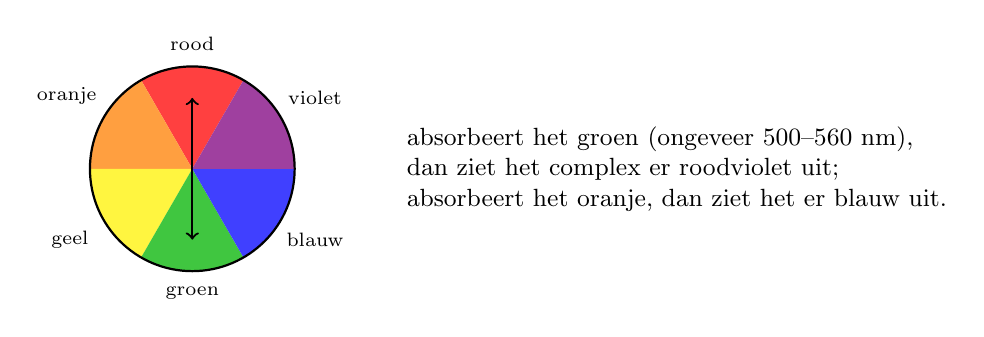
\begin{tikzpicture}[font=\scriptsize]
  \foreach \a/\c/\n in {90/red/rood, 150/orange/oranje, 210/yellow/geel, 270/green!70!black/groen, 330/blue/blauw, 30/violet/violet} {
    \fill[\c!75] (0,0) -- (\a-30:1.3) arc[start angle=\a-30, end angle=\a+30, radius=1.3] -- cycle;
    \node[anchor=\a+180] at (\a:1.38) {\n};
  }
  \draw[thick] (0,0) circle (1.3);
  \draw[<->, thick] (90:0.9) -- (270:0.9);
  \node[anchor=west, font=\small, align=left] at (2.6,0) {absorbeert het groen (ongeveer 500--560 nm),\\ dan ziet het complex er roodviolet uit;\\ absorbeert het oranje, dan ziet het er blauw uit.};
\end{tikzpicture}

{\small Een kleurencirkel: de waargenomen kleur is ruwweg de complementaire, diametraal
tegenover de geabsorbeerde band.}
\end{omfigure}

\begin{definition}[Spectrochemische reeks]\label{def:b2:ligand-field:spectrochemical}
De \emph{spectrochemische reeks}\index{spectrochemische reeks} rangschikt liganden naar de
splitsing die ze voor een gegeven metaalion veroorzaken:
\[
  \ce{I-} < \ce{Br-} < \ce{Cl-} < \ce{F-} < \ce{OH-} < \ce{H2O} < \ce{NH3} < \text{en} <
  \ce{NO2-} < \ce{CN-} < \ce{CO} .
\]
Voor een gegeven ligand groeit $\Delta_o$ ook met de lading van het metaalion en naar beneden in een groep
(4d- en 5d-complexen, groter dan 3d-complexen, zijn bijna altijd \omterm{def:b2:ligand-field:spin}{laagspin}).
\end{definition}

De halogeniden staan aan het zwakke uiteinde en \ce{CN-} en \ce{CO} aan het sterke, wat het
\omterm{def:b2:ligand-field:crystal-field}{kristalveldmodel} niet kan verklaren: het zou het geladen \ce{F-} boven het neutrale
\ce{CO} plaatsen. De verklaring vereist orbitalen.

\section{Het ligandveld}

\begin{definition}[Ligandveldtheorie]\label{def:b2:ligand-field:ligand-field}
De \emph{ligandveldtheorie}\index{ligandveldtheorie} beschrijft een complex met \omterm{def:b2:diatomic-mos:lcao}{molecuulorbitalen}
die opgebouwd zijn uit de valentieorbitalen van het metaal (zijn negen $n$d-, $(n+1)$s- en $(n+1)$p-orbitalen)
en de donororbitalen van de liganden.
\end{definition}

\begin{proposition}[$\sigma$-binding in een octaëdrisch complex]\label{prop:b2:ligand-field:mo-octahedral}
Met zes liganden die elk één $\sigma$-donororbitaal leveren, ontstaan zes bindende \omterm{def:b2:diatomic-mos:lcao}{molecuulorbitalen}
uit de s-, de drie p- en de twee $e_g$-orbitalen van het metaal; de drie $t_{2g}$-orbitalen, die
tussen de liganden door wijzen, blijven niet-bindend; daarboven liggen de antibindende $e_g^*$-orbitalen.
De elektronen van de liganden vullen de zes \omterm{def:b2:diatomic-mos:bonding}{bindende orbitalen}; de d-elektronen van het metaal gaan
naar $t_{2g}$ en $e_g^*$, gescheiden door $\Delta_o$. Bindende plus \omterm{def:b2:diatomic-mos:bonding}{niet-bindende orbitalen} kunnen
$12 + 6 = 18$ elektronen bevatten.
\end{proposition}

\begin{proof}[Redenering]
Volgens de fragmentmethode van \cref{ch:b2:fragment-orbitals} wisselwerkt elke metaalorbitaal
met de combinatie van ligandorbitalen van dezelfde symmetrie: s met de volledig
symmetrische, elke p met een paar tegenover elkaar liggende liganden, $\mathrm d_{z^2}$ en $\mathrm
d_{x^2-y^2}$ met de combinaties die langs hun lobben wijzen; geen enkele $\sigma$-combinatie
past bij de $t_{2g}$-orbitalen (hun overlap met elke $\sigma$-donor die langs een as wijst,
is door symmetrie nul). De namen van de combinaties komen uit de groepentheorie, aangenomen.
Alle bindende en \omterm{def:b2:diatomic-mos:bonding}{niet-bindende orbitalen} vullen, en geen van de antibindende, vergt
18 elektronen --- de \omterm{def:b2:coordination-complexes:electron-count}{18-elektronenregel}.
\end{proof}

\begin{omfigure}
\begin{tikzpicture}[font=\scriptsize]
  % metal
  \pic (m4p1) at (-0.45,2.6) {omlevel={empty}{0.4}}; \pic (m4p2) at (0,2.6) {omlevel={empty}{0.4}}; \pic (m4p3) at (0.45,2.6) {omlevel={empty}{0.4}};
  \node[anchor=east] at (-0.7,2.6) {$(n{+}1)$p};
  \pic (m4s) at (0,1.8) {omlevel={empty}{0.6}}; \node[anchor=east] at (-0.35,1.8) {$(n{+}1)$s};
  \foreach \x in {-0.9,-0.45,0,0.45,0.9} \pic at (\x,0.6) {omlevel={empty}{0.4}};
  \coordinate (m3d) at (1.1,0.6); \node[anchor=east] at (-1.15,0.6) {$n$d};
  \node[font=\small] at (0,-2.9) {metaal};
  % ligands
  \foreach \x in {6.2,6.72,7.24,7.76,8.28,8.8} \pic at (\x,-0.9) {omlevel={ud}{0.36}};
  \coordinate (lig) at (6.0,-0.9);
  \node[font=\small] at (7.3,-2.9) {zes $\sigma$-donororbitalen};
  % MOs
  \pic (b1) at (3.6,-2.4) {omlevel={ud}{0.5}};
  \foreach \x in {3.0,3.6,4.2} \pic at (\x,-1.9) {omlevel={ud}{0.5}};
  \pic at (3.3,-1.45) {omlevel={ud}{0.5}}; \pic at (3.9,-1.45) {omlevel={ud}{0.5}};
  \foreach \x in {3.0,3.6,4.2} \pic at (\x,0.3) {omlevel={empty}{0.5}};
  \pic at (3.3,1.5) {omlevel={empty}{0.5}}; \pic at (3.9,1.5) {omlevel={empty}{0.5}};
  \pic at (3.6,3.1) {omlevel={empty}{0.5}};
  \foreach \x in {3.0,3.6,4.2} \pic at (\x,3.6) {omlevel={empty}{0.5}};
  \node[anchor=north] at (3.6,0.12) {$t_{2g}$ (niet-bindend)};
  \node[anchor=west] at (4.2,1.5) {$e_g^*$};
  \node[anchor=north] at (3.6,-2.58) {6 bindend};
  \draw[<->, omProp] (2.55,0.3) -- (2.55,1.5) node[midway, right] {$\Delta_o$};
  \draw[omcorr, densely dashed] (m3d) -- (2.75,0.3) (m3d) -- (3.05,1.5) (1.1,0.6) -- (3.05,-1.45);
  \draw[omcorr, densely dashed] (lig) -- (4.15,-1.45) (lig) -- (4.45,-1.9) (lig) -- (3.85,-2.4) (lig) -- (4.15,1.5);
  \draw[omcorr, densely dashed] (m4s-r) -- (3.35,-2.4) (m4s-r) -- (3.35,3.1) (m4p3-r) -- (2.75,-1.9) (m4p3-r) -- (2.75,3.6);
\end{tikzpicture}

{\small \omterm{def:b2:diatomic-mos:lcao}{Molecuulorbitalen} van een octaëdrisch complex met zes $\sigma$-donoren,
schematisch. De twaalf elektronen van de liganden vullen de zes \omterm{def:b2:diatomic-mos:bonding}{bindende orbitalen}; de d-elektronen
van het metaal bezetten het niet-bindende niveau $t_{2g}$ en het antibindende $e_g^*$, gescheiden door
$\Delta_o$ --- het kristalveldbeeld teruggevonden. Tot 18 elektronen vullen de bindende en
niet-bindende niveaus.}
\end{omfigure}

\begin{definition}[$\pi$-donor- en $\pi$-acceptorliganden]\label{def:b2:ligand-field:pi-ligands}
Een \emph{$\pi$-donorligand}\index{pi-donorligand@$\pi$-donorligand} heeft gevulde orbitalen
met $\pi$-symmetrie ten opzichte van de binding metaal-ligand (vrije elektronenparen van \ce{Cl-},
\ce{OH-}); een \emph{$\pi$-acceptorligand}\index{pi-acceptorligand@$\pi$-acceptorligand}
heeft lege orbitalen met lage energie (de $\pi^*$-orbitalen van \ce{CO} en \ce{CN-}). De overdracht van
elektronendichtheid van gevulde d-orbitalen van het metaal naar de lege $\pi^*$-orbitalen van een
$\pi$-acceptorligand heet \emph{terugdonatie}\index{terugdonatie}.
\end{definition}

\begin{proposition}[$\pi$-effecten op de splitsing]\label{prop:b2:ligand-field:pi-effects}
$\pi$-donorliganden verkleinen $\Delta_o$; $\pi$-acceptorliganden vergroten haar.
\end{proposition}

\begin{proof}
De $t_{2g}$-orbitalen hebben de juiste symmetrie om met $\pi$-orbitalen van liganden te overlappen. Een gevulde
$\pi$-orbitaal van een ligand ligt onder $t_{2g}$: volgens \cref{thm:b2:frontier-orbitals:perturbation} duwt de
wisselwerking $t_{2g}$ omhoog, naar $e_g^*$, en wordt $\Delta_o$ kleiner. Een lege $\pi^*$-orbitaal
ligt boven $t_{2g}$: de wisselwerking duwt $t_{2g}$ omlaag, en $\Delta_o$ wordt groter. Het tweede geval
draagt d-dichtheid van het metaal over naar de $\pi^*$ van het ligand: \omterm{def:b2:ligand-field:pi-ligands}{terugdonatie}.
\end{proof}

\begin{omfigure}
\begin{tikzpicture}[font=\scriptsize]
  \begin{scope}
    \pic (t) at (0,1.2) {omlevel={empty}{0.6}}; \node[anchor=east] at (-0.35,1.2) {$t_{2g}$};
    \pic (l) at (2.4,0) {omlevel={ud}{0.6}}; \node[anchor=west] at (2.75,0) {ligand-$\pi$ (gevuld)};
    \pic (n) at (1.2,1.75) {omlevel={empty}{0.6}};
    \draw[omcorr, densely dashed] (t-r) -- (n-l) (l-l) -- (n-r);
    \pic (e) at (1.2,3.0) {omlevel={empty}{0.6}}; \node[anchor=west] at (1.55,3.0) {$e_g^*$};
    \draw[<->, omProp] (0.55,1.75) -- (0.55,3.0) node[midway, left] {$\Delta_o$ kleiner};
    \node[font=\small] at (1.2,-0.8) {$\pi$-donor};
  \end{scope}
  \begin{scope}[xshift=6.5cm]
    \pic (t) at (0,1.2) {omlevel={empty}{0.6}}; \node[anchor=east] at (-0.35,1.2) {$t_{2g}$};
    \pic (l) at (2.4,2.6) {omlevel={empty}{0.6}}; \node[anchor=west] at (2.75,2.6) {ligand-$\pi^*$ (leeg)};
    \pic (n) at (1.2,0.65) {omlevel={empty}{0.6}};
    \draw[omcorr, densely dashed] (t-r) -- (n-l) (l-l) -- (n-r);
    \pic (e) at (1.2,3.0) {omlevel={empty}{0.6}}; \node[anchor=west] at (1.55,3.15) {$e_g^*$};
    \draw[<->, omProp] (0.55,0.65) -- (0.55,3.0) node[midway, left] {$\Delta_o$ groter};
    \node[font=\small] at (1.2,-0.8) {$\pi$-acceptor (terugdonatie)};
  \end{scope}
\end{tikzpicture}

{\small Invloed van de $\pi$-orbitalen van liganden op het niveau $t_{2g}$, schematisch. Een gevulde
$\pi$-orbitaal eronder duwt $t_{2g}$ omhoog (kleinere splitsing); een lege $\pi^*$-orbitaal erboven trekt het
omlaag (grotere splitsing).}
\end{omfigure}

Dit plaatst \ce{CO} en \ce{CN-}, sterke $\sigma$-donoren en $\pi$-acceptoren, bovenaan de
\omterm{def:b2:ligand-field:spectrochemical}{spectrochemische reeks}, en de halogeniden, $\pi$-donoren, onderaan. Metaalcarbonylen hebben
hun $t_{2g}$-orbitalen gestabiliseerd en gevuld: de 18-elektronencomplexen van
\cref{ch:b2:coordination-complexes}.

\section{Oefeningen}

\begin{exercise}[$\star$]\label{exo:b2:ligand-field:1}
Geef de octaëdrische configuratie en de CFSE van een $d^3$-ion en van een $d^8$-ion.
\end{exercise}

\begin{exercise}[$\star$]\label{exo:b2:ligand-field:2}
Hoeveel ongepaarde elektronen hebben \ce{[Fe(H2O)6]^2+} (\omterm{def:b2:ligand-field:spin}{hoogspin}) en \ce{[Fe(CN)6]^4-}
(\omterm{def:b2:ligand-field:spin}{laagspin})?
\end{exercise}

\begin{exercise}[$\star$]\label{exo:b2:ligand-field:3}
Een complex absorbeert het sterkst bij \qty{600}{nm}. Welke kleur heeft het?
\end{exercise}

\begin{exercise}[$\star$]\label{exo:b2:ligand-field:4}
Rangschik \ce{H2O}, \ce{CN-}, \ce{Cl-}, \ce{NH3} naar de splitsing die ze veroorzaken.
\end{exercise}

\begin{exercise}[$\star\star$]\label{exo:b2:ligand-field:5}
Voor een $d^5$-ion is $\Delta_o = \qty{165}{kJ/mol}$ met water en $\qty{390}{kJ/mol}$ met cyanide,
en $P = \qty{300}{kJ/mol}$ (gegevens voor de oefening). Voorspel beide spintoestanden en de ongepaarde
elektronen.
\end{exercise}

\begin{exercise}[$\star\star$]\label{exo:b2:ligand-field:6}
\ce{[Co(H2O)6]^2+} is roze, \ce{[CoCl4]^2-} diepblauw. Verklaar de kleurverandering uit de
verandering van geometrie en ligand.
\end{exercise}

\begin{exercise}[$\star\star$]\label{exo:b2:ligand-field:7}
Toon aan dat het vlak vierkante \ce{[Ni(CN)4]^2-} \omterm{def:b2:diatomic-mos:magnetism}{diamagnetisch} is, terwijl het tetraëdrische
\ce{[NiCl4]^2-} twee ongepaarde elektronen heeft.
\end{exercise}

\begin{exercise}[$\star\star$]\label{exo:b2:ligand-field:8}
Een $d^1$-complex absorbeert bij \qty{500}{nm} (gegevens voor de oefening). Bereken $\Delta_o$ in \unit{cm^{-1}} en
\unit{kJ/mol}.
\end{exercise}

\begin{exercise}[$\star\star$]\label{exo:b2:ligand-field:9}
Waarom zijn verbindingen van \ce{Zn^2+} en \ce{Sc^3+} kleurloos?
\end{exercise}

\begin{exercise}[$\star\star\star$]\label{exo:b2:ligand-field:10}
Tel de elektronen in de \omterm{def:b2:diatomic-mos:lcao}{molecuulorbitalen} van \ce{[Co(NH3)6]^3+}: welke niveaus zijn gevuld,
en is het complex \omterm{def:b2:diatomic-mos:magnetism}{diamagnetisch}?
\end{exercise}

\begin{exercise}[$\star\star\star$]\label{exo:b2:ligand-field:11}
Leg uit waarom \ce{CO}, een neutraal en zwak basisch molecuul, een grotere splitsing geeft dan
het fluoride-ion.
\end{exercise}

\begin{exercise}[$\star\star\star$]\label{exo:b2:ligand-field:12}
De hydratatie-enthalpieën van de ionen \ce{M^2+} van \ce{Ca^2+} tot \ce{Zn^2+}, uitgezet tegen $n$, vormen
twee bulten boven een rechte door $d^0$, $d^5$ en $d^{10}$. Verklaar de vorm met de
CFSE bij \omterm{def:b2:ligand-field:spin}{hoogspin}.
\end{exercise}

\section{Probleem: rode robijn, groene smaragd}

\begin{problem}[{Weekendprobleem --- chroom(III) in een octaëdrisch veld, de absorptiebanden
van robijn en de kleur die ze overlaten, het zwakkere veld van smaragd, en gehydrateerd en
watervrij kopersulfaat}]
\label{pb:b2:ligand-field:1}
Gegevens voor het probleem (afgerond, illustratief): robijn (\ce{Cr^3+} in \ce{Al2O3}) absorbeert
in twee banden, rond \qty{556}{nm} en \qty{405}{nm}; in smaragd (\ce{Cr^3+} in beril) ligt de
eerste band rond \qty{620}{nm}. Voor een $d^3$-ion komt de eerste band overeen met
$\Delta_o$. $N_Ahc = \qty{0.1196}{J.m/mol}$.
% ledger: const:NA, const:h, const:c

\medskip
\noindent\textbf{Deel I --- Chroom(III).}
\begin{enumerate}
  \item Geef de $d^n$-configuratie van \ce{Cr^3+}.
  \item Hoe is ze verdeeld in een octaëdrisch veld?
  \item Is er een keuze tussen \omterm{def:b2:ligand-field:spin}{hoogspin} en \omterm{def:b2:ligand-field:spin}{laagspin}?
  \item Bereken haar CFSE.
  \item Hoeveel ongepaarde elektronen heeft het ion?
  \item Waarom zijn chroom(III)complexen kinetisch inert (wisselen ze traag liganden uit)?
\end{enumerate}

\medskip
\noindent\textbf{Deel II --- Robijn.}
\begin{enumerate}[resume]
  \item Wat omringt een \ce{Cr^3+}-ion dat in korund de plaats van \ce{Al^3+} inneemt?
  \item Reken de eerste band om naar een golfgetal.
  \item Leid $\Delta_o$ af in \unit{kJ/mol}.
  \item Welke kleuren worden door de twee banden geabsorbeerd?
  \item Wat blijft er over om gezien te worden?
  \item Waarom zijn er twee banden voor één enkele splitsing? (Een kwalitatief antwoord.)
\end{enumerate}

\medskip
\noindent\textbf{Deel III --- Smaragd.}
\begin{enumerate}[resume]
  \item Reken de band van smaragd om naar $\Delta_o$.
  \item Vergelijk met robijn: welk kristal geeft het sterkste veld?
  \item Waarheen verschuift de geabsorbeerde kleur, en welke kleur wordt doorgelaten?
  \item Opper een structurele reden voor het zwakkere veld in beril.
  \item Zou het aantal ongepaarde elektronen veranderen?
\end{enumerate}

\medskip
\noindent\textbf{Deel IV --- Kopersulfaat.}
\begin{enumerate}[resume]
  \item Wat is de configuratie van \ce{Cu^2+}?
  \item In \ce{CuSO4.5H2O} is koper omringd door watermoleculen. Waarom is de vaste stof blauw?
  \item Wat gebeurt er met de kleur wanneer het water verdreven wordt, en waarom?
  \item Waarom maakt een druppel water het witte poeder weer blauw?
  \item Zou \ce{[Cu(NH3)4]^2+} bij een kortere of langere golflengte absorberen dan het aqua-ion?
  \item Kan een $d^9$-ion \omterm{def:b2:ligand-field:spin}{hoogspin} of \omterm{def:b2:ligand-field:spin}{laagspin} zijn?
  \item Is \ce{CuSO4.5H2O} \omterm{def:b2:diatomic-mos:magnetism}{paramagnetisch}?
  \item Geef $\Delta_o$ van \ce{Cr^3+} in robijn uit zijn eerste absorptieband.
\end{enumerate}
\end{problem}
